\documentclass[xcolor={dvipsnames,rgb}, aspectratio=169]{beamer}

%%% PACKAGES %%%
\usepackage[T1]{fontenc}
\usepackage{tgheros}

% Metropolis customization
\usetheme[sectionpage=none]{metropolis}
\setbeamercolor{background canvas}{bg=white}
\setbeamercolor{frametitle}{bg = white, fg=black}
\setbeamertemplate{sections/subsections in toc}[square]
\setbeamertemplate{footline}{
   \textcolor{bluepoli}{\rule{\paperwidth}{1pt}}
   \vskip4pt
   \hskip5pt \tiny Linear System Of Equations (Pt. 2) $|$ Calcoli di Processo dell' Ingegneria
   Chimica \hskip220pt \insertframenumber
   \vskip4pt
}

% color
\usepackage{color}
\usepackage{xcolor}
\usepackage{colortbl}
\definecolor{bluepoli}{cmyk}{0.4,0.1,0,0.4}
\definecolor{mygreen}{RGB}{1, 121,111}
\definecolor{myred}{RGB}{220, 20, 60}
\definecolor{mygreen}{RGB}{28,172,0}
\definecolor{mylilas}{RGB}{170,55,241}
\definecolor{codegreen}{rgb}{0,0.6,0}
\definecolor{codegray}{rgb}{0.5,0.5,0.5}
\definecolor{codepurple}{rgb}{0.58,0,0.82}
\definecolor{backcolour}{rgb}{0.95,0.95,0.92}
\definecolor{lightblue}{rgb}{56, 167, 232}

\colorlet{colorp}{NavyBlue}
\colorlet{colorT}{WildStrawberry}
\colorlet{colork}{OliveGreen}
\colorlet{colorM}{RoyalPurple}
\colorlet{colorNb}{Plum}
\colorlet{colorIs}{black}
\newcommand{\highlight}[2]{\colorbox{#1!17}{$#2$}}
\newcommand{\highlightdark}[2]{\colorbox{#1!47}{$#2$}}

% tikz
\usepackage{tikz}
\usetikzlibrary{positioning}
\usetikzlibrary{backgrounds}
\usetikzlibrary{arrows,shapes}
\usetikzlibrary{tikzmark}
\usetikzlibrary{calc}

% tcolorbox env
% Coloured box for styling theorems, proof, definitions
\usepackage[most]{tcolorbox}

\newtcolorbox{code}[2][]{
    enhanced jigsaw,
    colframe=bluepoli,
    interior hidden, 
    breakable,
    before skip=10pt,
    after skip=10pt
}

% URL and Hyperref
\usepackage{hyperref}
\hypersetup{
    colorlinks=true,
    linkcolor=blue,
    filecolor=magenta,
    urlcolor=blue,
    pdftitle={Overleaf Example},
    pdfpagemode=FullScreen,
}
\usepackage{url}

% Math stuff
\usepackage{amsmath}
\usepackage{amssymb}
\usepackage{mathtools}
\usepackage{blkarray}
\usepackage{multirow}

% Wrapfig
\usepackage{wrapfig}

% Bibliography
\usepackage[
backend=biber,
style=alphabetic,
sorting=ynt
]{biblatex}
\addbibresource{bibliography.bib}

%%% TITLE %%%
\title{Linear System Of Equations.\\Part 2}
\subtitle{Calcoli di Processo dell' Ingegneria Chimica}
\author[Dinelli, Mehl]{\textbf{Timoteo~Dinelli}, \textbf{Marco~Mehl}}
\institute{
   \inst{} Department of Chemistry, Materials and Chemical Enginering, G. Natta.
   Politecnico di Milano.\\
   email: timoteo.dinelli@polimi.it \\
   email: marco.mehl@polimi.it \\
}
\date{24\textsuperscript{th} of October 2024.}

\begin{document}
% external files inclusion
% Double underline
\def\doubleunderline#1{\underline{\underline{#1}}}

% \newcommand{\zm}{%
%    \begin{bmatrix}
%       X_{11} & X_{12} & \cdots & X_{1p} \\
%       X_{12} & X_{22} & \cdots & X_{2p} \\
%       \vdots & \vdots & \tikzmarknode{Is}{\highlight{colorT}{X_{ij}}} & \vdots \\
%       X_{n1} & X_{n2} & \cdots & X_{np} \\
%    \end{bmatrix}%
% }

\makeatletter
\newcommand{\DrawLine}{%
  \begin{tikzpicture}
  \path[use as bounding box] (0,0) -- (\linewidth,0);
  \draw[color=bluepoli,dashed,dash phase=2pt]
        (0-\kvtcb@leftlower-\kvtcb@boxsep,0)--
        (\linewidth+\kvtcb@rightlower+\kvtcb@boxsep,0);
  \end{tikzpicture}%
  }
\makeatother

{%
   \setbeamertemplate{footline}{}
   \begin{frame}{}
      \maketitle
      \begin{tikzpicture}[overlay, remember picture]
         \node[above left=6.5cm and .01cm of current page.south east] {
         \includegraphics[trim=1cm 1cm 1.5cm 1cm, clip=true, width=6cm]{
            ./../../Introduction to Matlab/slides/figures/_static/ING_IND_INF-eps-converted-to.pdf
         }
      };
      \end{tikzpicture}
   \end{frame}
}

\begin{frame}{Linear System Of Equations}
   \small{In mathematics, and particularly in linear algebra, a system of linear
   equations, also called a linear system, is a system composed of several \alert{linear
   equations} that must all be verified simultaneously. A solution of the system is a
   vector whose elements are the solutions of the equations that make up the system, that
   is, such that when substituted for the unknowns make the equations identities.}

   From the classical representation to the \alert{\textbf{matricial}} form:
   \begin{equation*}
      \tikzmarknode{Amatrix}{\highlight{colork}{
         \begin{bmatrix}
            a_{1,1} & a_{1,2} & \ldots & a_{1,n} \\
            a_{2,1} & a_{2,2} & \ldots & a_{2,n} \\
            \vdots  & \vdots  & \ddots & \vdots  \\
            a_{n,1} & a_{n,2} & \ldots & a_{n,n}
         \end{bmatrix}
      }}\:
      \tikzmarknode{xvector}{\highlight{colorp}{
         \begin{bmatrix}
            x_{1}  \\
            x_{2}  \\
            \vdots \\
            x_{n}
         \end{bmatrix}
      }}
      =
      \tikzmarknode{xvector}{\highlight{colorT}{
         \begin{bmatrix}
            b_{1}  \\
            b_{2}  \\
            \vdots \\
            b_{n}
         \end{bmatrix}
      }}
   \end{equation*}

   \begin{equation*}
      \textcolor{colork}{\textbf{\underline{\underline{A}}}} \:
      \textcolor{colorp}{\textbf{\underline{x}}} =
      \textcolor{colorT}{\textbf{\underline{b}}}
      \quad \longrightarrow \quad
      \textbf{\underline{x}} = \textbf{\underline{\underline{A}}}^{\textbf{-1}} \:
      \textbf{\underline{b}}
   \end{equation*}
\end{frame}

\begin{frame}{Problem!?}

   What if the element on which we have to compute the coefficient for the factorization is
   equal to zero?\\

   \Huge \textbf{PIVOTING!} \\

   \normalsize We call \textbf{\textit{pivot}} the first non-zero element encountered in
   each row in a stepped matrix.

   \begin{equation*}
      A = 
         \begin{bmatrix}
            0 & 5 & 7 & 4 \\
            0 & 0 & -2 & 0 \\
            0 & 0 & 0 & 22
         \end{bmatrix}
   \end{equation*}
   \begin{equation*}
      a_{1,2} = 5; \quad a_{2,3} = -2; \quad a_{3,4} = 22
   \end{equation*}
\end{frame}

\begin{frame}{Pivoting(s)}
   \vspace{-.5cm}
   \alert{Trivial Pivoting}:\\
   if $a_{k,k}^{(k-1)} = 0$ take the first row $p$ under the row $k$ for which the
   element $a_{p,k}^{(k-1)} \neq 0$ then we will swap the row $p$ with the row $k$.\\
   \alert{Global Pivoting}:\\
   At the $k-th$ iteration the pivot is the maximum coefficient among all the ones that
   are left.
   \begin{equation*}
      |a_{p,q}^{(k-1)}| = \underset{k<i<n,k<j<n}{\mathrm{max}}\left(|a_{i,j}^{(k-1)}|\right)
   \end{equation*}

   \footnotesize{
      \begin{itemize}
         \item[$\blacktriangleright$] If $p \neq k$ the row $p$ is swapped with the row
            $k$.
         \item[$\blacktriangleright$] If $q \neq k$ the column $q$ is swapped with the
            column $k$
         \item[$\blacktriangleright$] If the rows are swapped, then the elements of the
            constant terms \textbf{b} are also swapped accordingly
         \item[$\blacktriangleright$] If the columns are swapped, then the elements of
            the unknown \textbf{x} are also swapped accordingly.
      \end{itemize}
   }
\end{frame}

\begin{frame}{}
   \alert{Partial Pivoting}:\\
   at the $k-th$ iteration the pivot is the maximum coefficient among the elements in the
   $k-th$ column:
   \begin{equation*}
      |a_{p,q}^{(k-1)}| = \underset{k<i<n}{\mathrm{max}}\left(|a_{i,k}^{(k-1)}|\right)
   \end{equation*}

   \begin{itemize}
      \item If $p \neq k$ the row $p$ is swapped with the row $k$.
      \item If the rows are swapped, then the elements of the constant terms \textbf{b}
         are also swapped accordingly.
   \end{itemize}

   The \alert{\textbf{global pivot}} is the most effective strategy for limiting the
   numerical errors, the \alert{\textbf{partial pivot}} does not guarantee the same
   accuracy. Often, though, the difference between the two is often negligible so the
   partial pivot is generally preferred because of the lower computational burden.
\end{frame}

\begin{frame}{}
   \alert{Scaled Partial Pivoting}:\\
   At the $k-th$ iteration the index $p$ is determined:
   \begin{equation*}
      |a_{p,k}^{(k-1)}| =
      \underset{k<i<n}{\mathrm{max}}\frac{|a_{i,k}^{(k-1)}|}{\underset{k<j<n}{\mathrm{max}}|a_{i,j}^{(k-1)}|}
   \end{equation*}
   If $p \neq k$ the row $p$ is swapped with the row $k$ without doing any further
   balancing which can introduce other rounding errors. The key step is then finding the
   index $p$ which determines the optimal pivot.\\ \textbf{Applying a further balancing
   potentially can introduce additional unnecessary rounding errors that could be
   potentially cancel out all the benefits gained by the balancing itself.}
\end{frame}

{%
   \setbeamertemplate{footline}{}
   \begin{frame}[standout]
	   Exercises
   \end{frame}
}
\begin{frame}{}
   \begin{itemize}
      \item[$\blacktriangleright$] Write a MATLAB function to perform the Gauss
         Elimination with partial pivoting.
      \item[$\blacktriangleright$] Write a MATLAB function to perform the Gauss
         Elimination with balanced partial pivoting.
      \item[$\blacktriangleright$] Given the system of equations reported below:
         \begin{equation*}
            \begin{bmatrix}
               1   & 2  & 3 \\
               40  & 50 & 60 \\
               160 & 25 & 30
            \end{bmatrix}
            \begin{bmatrix}
               x_{1} \\ x_{2} \\ x_{3}
            \end{bmatrix} =
            \begin{bmatrix}
               1 \\ 1 \\ 1
            \end{bmatrix}
         \end{equation*}
         Solve it employing the Gauss elimination method with and without partial
         pivoting paying attention to employ two significant figures. And compare the
         solution in double precision with the one obtained with MATLAB
         $\left(x_{1}=0.0036; x_{2}=-1.9071;x_{3}=1.6036\right)$
   \end{itemize}
\end{frame}

\begin{frame}{}
   \begin{itemize}
      \item[$\blacktriangleright$] Chloride, often used as an indicator of pollution, has
         increased in concentration throughout the Great Lakes during the past century.
         Let's write a Matlab program that estimates the concentration of chloride in the
         Great Lakes given the following data.
         \begin{figure}
            \centering
            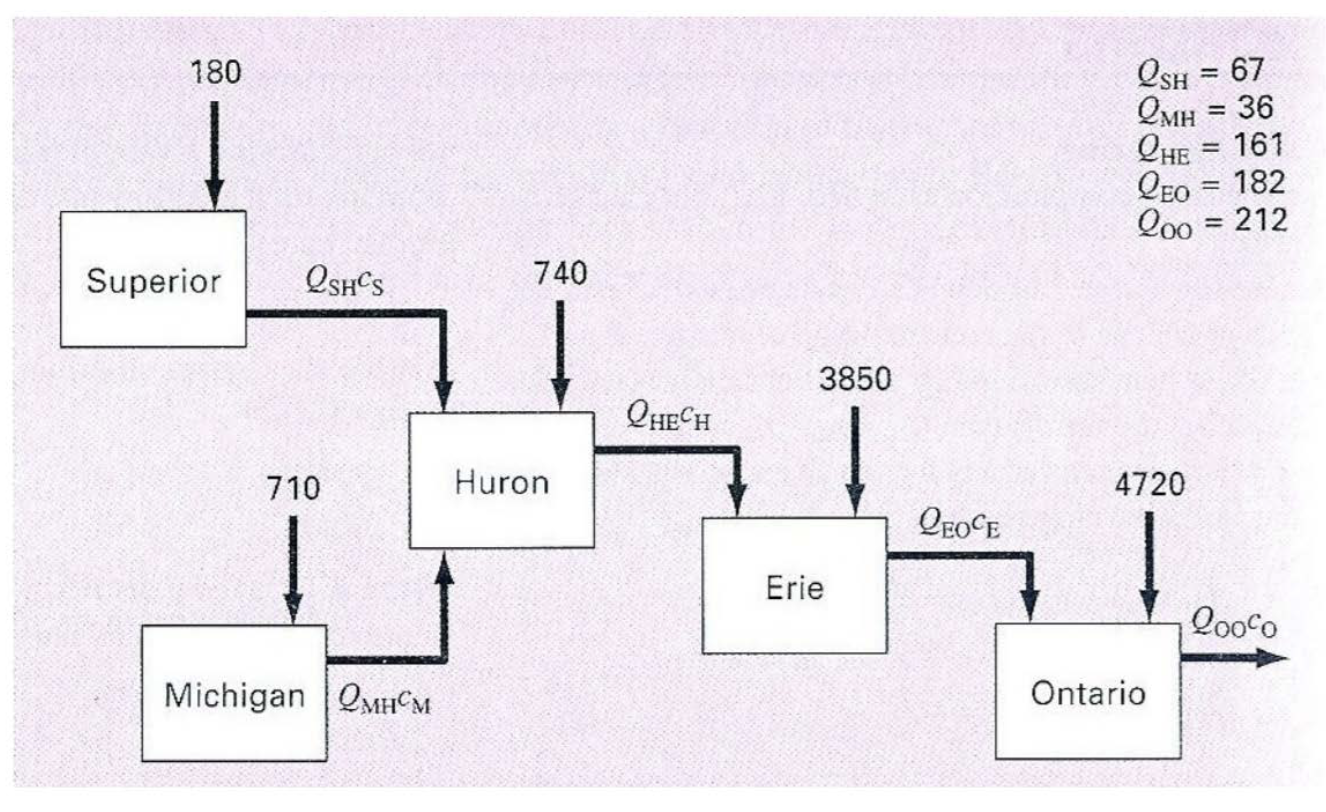
\includegraphics[width=0.6\textwidth]{figures/lakes.png}
         \end{figure}
   \end{itemize}
\end{frame}

\begin{frame}{}
   \begin{table}
   \centering
   \begin{tabular}{l|l|l|l}
      & \textbf{OutFlow [$Gm^{3}/year$]} & \textbf{Chloride load [$tonn/year$]} & \textbf{Volume [$km^{3}$]}  \\
      \hline
      \textbf{Superior} & 67  & 180  & 12000 \\
      \textbf{Michigan} & 36  & 710  & 4900  \\
      \textbf{Huron}    & 161 & 740  & 3500  \\
      \textbf{Erie}     & 182 & 3850 & 480   \\
      \textbf{Ontario}  & 212 & 4720 & 1640
   \end{tabular}
   \end{table}
\end{frame}

\begin{frame}{}
   \begin{columns}
      \column{0.5\textwidth}
      \begin{itemize}
         \item[$\blacktriangleright$] A Perfectly Stirred Reactor (PSR) is a type of
            continuous reactor characterized by a uniform internal composition,
            maintained through perfect mixing. Consequently, the composition of the
            exiting stream is identical to that within the reactor. At steady-state
            operation, the species balance for component \textit{i} can be expressed
            through the following equation:
            \begin{equation*}
               Q_{in}C_{i}^{0} - Q_{out}C_{i} = \nu_{i}RV
            \end{equation*}
      \end{itemize}
      \column{0.5\textwidth}
      \begin{figure}
         \centering
         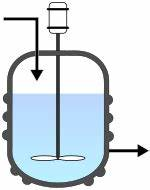
\includegraphics[width=0.6\textwidth]{Figures/proxy.jpeg}
      \end{figure}
   \end{columns}
\end{frame}

\begin{frame}{}
   \begin{itemize}
      \item[ ] Here, $R$ represents the cumulative sum of all rates of formation or
         destruction, adjusted by the appropriate coefficients. If the density remains
         constant, the equations can be formulated as follows:
         \begin{equation*}
            \frac{C_{i}^{0}-C_{i}}{\tau} = \nu_{i}R
         \end{equation*}
   \end{itemize}
   We will consider the following irreversible reactions taking place:
   \begin{itemize}
      \item[$\blacktriangleright$] $R1:\: A\longrightarrow B,\: K1=0.2$
      \item[$\blacktriangleright$] $R2:\: B\longrightarrow C,\: K2=0.1$
      \item[$\blacktriangleright$] $R3:\: B\longrightarrow D,\: K3=0.2$
      \item[$\blacktriangleright$] $R4:\: A\longrightarrow D,\: K4=0.3$
   \end{itemize}
\end{frame}

\begin{frame}{}
   Now the system to be solved is:\\
   \begin{equation*}
   \begin{cases}
      C_{A,0} = C_{A}\left(1+\tau K_{1} + \tau K_{4}\right) \\
      C_{B,0} = -C_{A}\left(\tau K_{1}\right) + C_{B}\left(1+\tau K_{2} + \tau K_{3}\right) \\
      C_{C,0} = -C_{B}\left(\tau K_{2}\right) + C_{C} \\
      C_{D,0} = -C_{A}\left(\tau K_{4}\right)-C_{B}\left(\tau K_{3}\right) + C_{D}
      C_{A,0} = C_{A}\left(1+\tau K_{1} + \tau K_{4}\right) \\
   \end{cases}
   \end{equation*}

   With $\tau = 1$s find the solution for the different inlet compositions reported
   below:
   \begin{table}
   \centering
   \begin{tabular}{l|l|l|l|l|l|l}
      & 1 & 2   & 3    & 4   & 5   & 6     \\
      \hline
      $C_{A,0}$ & 1 & 0.5 & 0.5  & 0.7 & 0.4 & 0.25  \\
      $C_{B,0}$ & 0 & 0.5 & 0.25 & 0.2 & 0.4 & 0.25  \\
      $C_{C,0}$ & 0 & 0   & 0.25 & 0   & 0.2 & 0.25  \\
      $C_{D,0}$ & 0 & 0   & 0    & 0.1 & 0   & 0.25
   \end{tabular}
   \end{table}
\end{frame}

\begin{frame}{}
   Now modify the script for the previous excersize in order to express the kinetic
   constant using the arrhenius formulation in a window of temperature between (450-650
   K):
   \begin{itemize}
      \item[$\blacktriangleright$] $K1 = 1e8 \times exp(-20000/1.987/T)$
      \item[$\blacktriangleright$] $K2 = 1e6 \times exp(-15000/1.987/T)$
      \item[$\blacktriangleright$] $K3 = 1e11 \times exp(-27000/1.987/T)$
      \item[$\blacktriangleright$] $K4 = 1e9 \times exp(-23000/1.987/T)$
   \end{itemize}
\end{frame}

%%%%%%%%%%%%%%% CLOSING
{%
\setbeamertemplate{footline}{}
\begin{frame}[standout]
	Thank you for the attention!
\end{frame}
}

\end{document}
